
\documentclass[letterpaper,11pt]{article}
\usepackage{graphicx}
\usepackage{listings}

\lstset{
	basicstyle=\footnotesize,
	breaklines=true,
}

\begin{document}

\begin{titlepage}

\begin{center}

\Huge{Assignment 3}

\Large{CS 532:  Introduction to Web Science}

\Large{Spring 2016}

\Large{Manoj Chandra Kompalli}

\Large Finished on February 18,2016

\end{center}

\end{titlepage}

\newpage
\section*{1}

\subsection*{Question}

\begin{verbatim}

1.  Download the 1000 URIs from assignment #2.  "curl", "wget", or
"lynx" are all good candidate programs to use.  We want just the
raw HTML, not the images, stylesheets, etc.
from the command line:

% curl http://www.cnn.com/ > www.cnn.com

% wget -O www.cnn.com http://www.cnn.com/

% lynx -source http://www.cnn.com/ > www.cnn.com

"www.cnn.com" is just an example output file name, keep in mind
that the shell will not like some of the characters that can occur
in URIs (e.g., "?", "&").  You might want to hash the URIs, like:

% echo -n "http://www.cs.odu.edu/show_features.shtml?72" | md5
41d5f125d13b4bb554e6e31b6b591eeb

("md5sum" on some machines; note the "-n" in echo -- this removes
the trailing newline.) 

Now use a tool to remove (most) of the HTML markup.  "lynx" will
do a fair job:

% lynx -dump -force_html www.cnn.com > www.cnn.com.processed
Use another (better) tool if you know of one.  Keep both files 
for each URI (i.e., raw HTML and processed). 

\end{verbatim}


\subsection*{Answer}

I had extracted all URIs from the second assignment in the same JSON format. I have then used the command
\begin{lstlisting}[frame=single]
curl -s -L  "URI"  >./rawurls/filename
\end{lstlisting}

to generate the raw html content into a directory.
I had also used the command below to generate processed URIs
\begin{lstlisting}[frame=single]
lynx -dump -force_html "URI" >./processedurls/ filename
\end{lstlisting}

I used the os library to execute shell commands from the python file.
I knew that I had to unique generate all 2000 URIs combined which could have either been done by using the md5 hashing technique you have mentioned in the question .
Just to improve the readability of the file names I decided to use a counter and count to 1000 and append that to a string each time for all 1000 URIs. I have used this approach for both the raw URIs and processed URIs.  



\subsection*{Code Listing} 
\lstinputlisting[language=Python, breaklines=true]{extract.py}
\begin{figure}
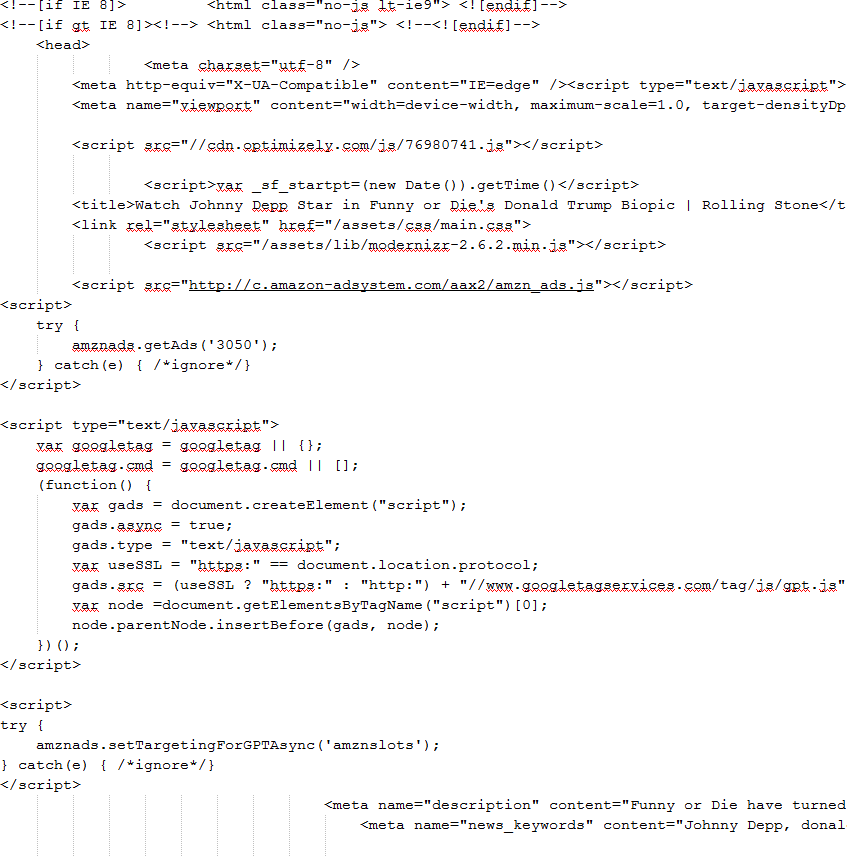
\includegraphics[scale=0.6]{sampleraw.png}
\caption{Images showing the raw html content generated for a URI}
\end{figure}
\begin{figure}
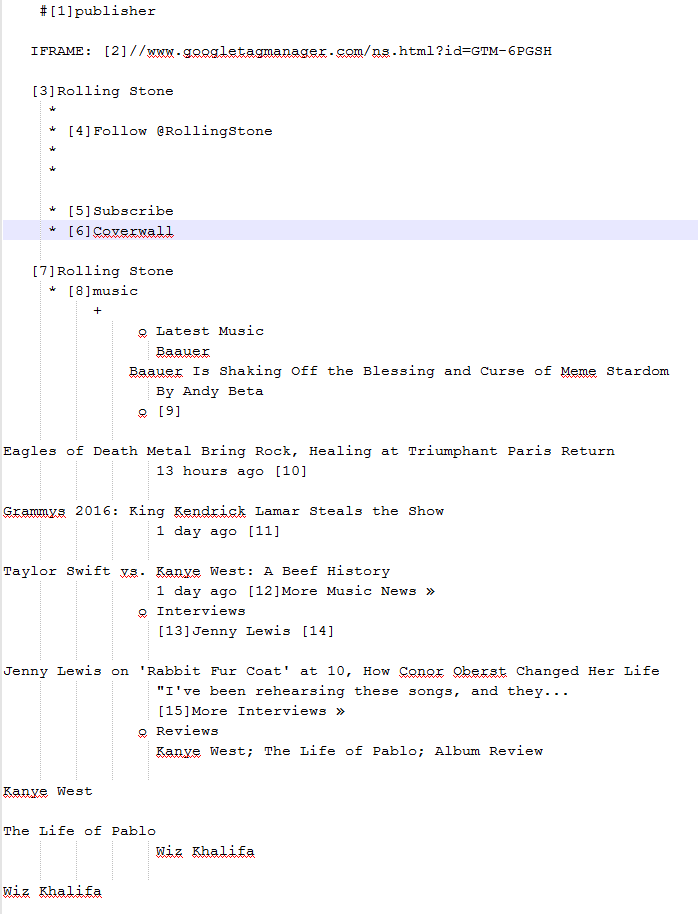
\includegraphics[scale=0.6]{sampleprocessed.png}
\caption{Response without html tags,stylesheets etc}

\end{figure}






\newpage
\section*{2}

\subsection*{Question}





\begingroup
\fontsize{8pt}{10pt}\selectfont
\begin{verbatim}
2.  Choose a query term (e.g., "shadow") that is not a stop word
(see week 5 slides) and not HTML markup from step 1 (e.g., "http")
that matches at least 10 documents (hint: use "grep" on the processed
files).  If the term is present in more than 10 documents, choose
any 10 from your list.  (If you do not end up with a list of 10
URIs, you've done something wrong).

As per the example in the week 5 slides, compute TFIDF values for
the term in each of the 10 documents and create a table with the
TF, IDF, and TFIDF values, as well as the corresponding URIs.  The
URIs will be ranked in decreasing order by TFIDF values.  For
example:

Table 1. 10 Hits for the term "shadow", ranked by TFIDF.

TFIDF	TF	IDF	URI
-----	--	---	---
0.150	0.014	10.680	http://foo.com/
0.044	0.008	 5.510	http://bar.com/


You can use Google or Bing for the DF estimation.  To count the
number of words in the processed document (i.e., the deonminator
for TF), you can use "wc":

% wc -w www.cnn.com.processed
    2370 www.cnn.com.processed

It won't be completely accurate, but it will be probably be
consistently inaccurate across all files.  You can use more 
accurate methods if you'd like.  

Don't forget the log base 2 for IDF, and mind your significant
digits!

\end{verbatim}
\endgroup


\newpage
\subsection*{Answer}
I had started off by trying to use grep command from the shell. I had figured out that grep could be used to find files with a keyword. I used keyword crime on the processed files.I used the following command to get all similar words matching keyword crime.
\begin{lstlisting}[frame=single]
 grep -lr "crime" directoryname
\end{lstlisting}
I got a few matching files from where I have randomly selected ten URIs.
\begin{lstlisting}[frame=single]
 'grep -c ' +'crime ' filename.
\end{lstlisting}
I used the command wc –w  to get the list of all words from a URI. I had then taken a ratio for the occurred words to total words which gave me TF.

For IDF I used the search results from Bing. Bing has a corpus value of 17 billion and queried word crime has 18 million search results. The ratio of the logarithm 

Log(corpus value/doc term) gives the IDF. The product of TF,IDF gives TFIDF.
I had measured the values for TFIDF .My next task was to arrange the tfidf values in descending order.
More TF-IDF value indicates more occurrence in that URI or less count of total words.


\subsection*{Code Listing} 
\lstinputlisting[language=Python, breaklines=true]{tfidf.py}
\newpage
\subsection*{Selected random ten files matching keyword} 
\lstinputlisting[language=Python, breaklines=true]{ten_files.txt}
\subsection*{TF,IDF,TF-IDF} 
\lstinputlisting[language=Python, breaklines=true]{tfidfsorted.txt}
\newpage

\section*{3}

\subsection*{Question}

\begin{verbatim}
3.  Now rank the same 10 URIs from question #2, but this time 
by their PageRank.  Use any of the free PR estimaters on the web,
such as:

http://www.prchecker.info/check_page_rank.php
http://www.seocentro.com/tools/search-engines/pagerank.html
http://www.checkpagerank.net/

If you use these tools, you'll have to do so by hand (they have
anti-bot captchas), but there is only 10.  Normalize the values
they give you to be from 0 to 1.0.  Use the same tool on all 10
(again, consistency is more important than accuracy).

Create a table similar to Table 1:

Table 2.  10 hits for the term "shadow", ranked by PageRank.

PageRank	URI
--------	---
0.9		http://bar.com/
0.5		http://foo.com/

Briefly compare and contrast the rankings produced in questions 2
and 3.



\end{verbatim}

\newpage
\subsection*{Answer}
I had used one of the web service http://www.seocentro.com/tools/search-engines/pagerank.html on all the ten URIs I was using for my previous problem. 


I had generated the page ranks for each URI and then sorted the URIs based on the page rank. 
 
 
 We can compare the page rank with the TF-IDF value even though it makes very little sense. Higher TF-IDF values had good page rank on an average. Higher page rank shows more traffic, keyword density, page authority  etc.I had used the shortened URIs because the complete URIs did not have less or no page rank at all.
 
\subsection*{Comparing Page Rank,TF-IDF of URIs } 
\lstinputlisting[language=Python, breaklines=true]{pagerank.txt}




\newpage

\section*{4}

\subsection*{Question}


\begin{verbatim}

4.  Compute the Kendall Tau_b score for both lists (use "b" because
there will likely be tie values in the rankings).  Report both the
Tau value and the "p" value.

See: 
http://stackoverflow.com/questions/2557863/measures-of-association-in-r-kendalls-tau-b-and-tau-c
http://en.wikipedia.org/wiki/Kendall_tau_rank_correlation_coefficient#Tau-b
http://en.wikipedia.org/wiki/Correlation_and_dependence
\end{verbatim}

\subsection*{Answer}
Kendall's Tau  gives the relation between TF-IDF and page rank. Tau Value closer to 1 denotes high correleation. Tau value 0 denotes no correlation .My TF-IDF and page rank vectors have given me a tau value of 0.906747. z=3.4603 ,p-value of 0.0002698.My results show that there is a lot of correlation between TF-IDF and Page Rank vectors.
\newpage
\subsection*{Program to find Tau value} 
\lstinputlisting[language=Python, breaklines=true]{kendall.R}
\begin{figure}
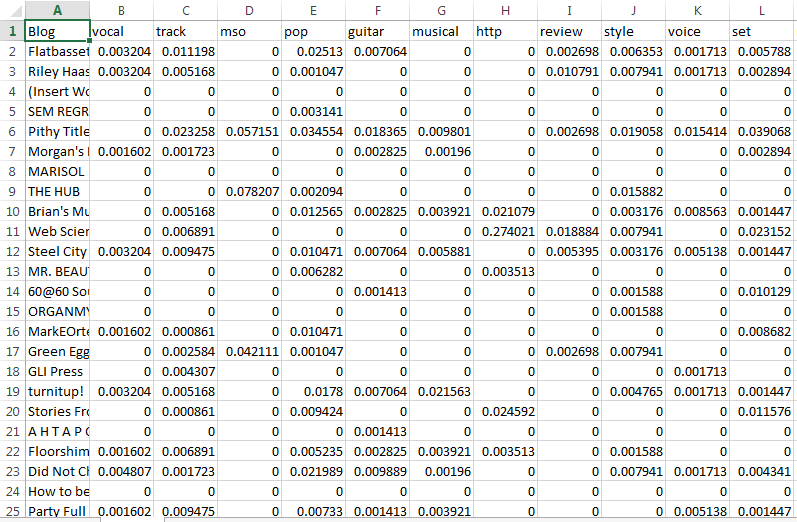
\includegraphics[scale=0.7]{output.png}
\caption{The output of the R console which gives Tau value}
\end{figure}
\newpage

\bibliographystyle{plain} 

\bibliography{references} 


\end{document}



